\documentclass[border=6pt]{standalone}
\usepackage{tikz}
\usetikzlibrary{arrows.meta,calc}

\definecolor{intfill}{RGB}{233,211,122}    % gold (internal element / container circles)
\definecolor{leaffill}{RGB}{200,216,242}   % light blue (node boxes)
\definecolor{nodeline}{RGB}{60,72,140}     % navy
\definecolor{elemcol}{RGB}{200,60,40}      % red element pointer
\definecolor{lettercol}{RGB}{150,70,30}    % brown element label

% General-tree node box: [ element | parent | children-ptr ]
% #1 x  #2 y  #3 letter  #4 parentflag(0=null,1=ptr)  #5 childflag(0=null,1=ptr)
% #6 element-cell fill colour
\newcommand{\gtbox}[6]{%
  \begin{scope}[shift={(#1,#2)}]
    \begin{scope}
      \clip[rounded corners=4pt] (-1.2,-0.35) rectangle (1.2,0.35);
      \fill[leaffill] (-1.2,-0.35) rectangle (1.2,0.35);
      \fill[#6] (-1.2,-0.35) rectangle (-0.4,0.35);
    \end{scope}
    \draw[nodeline, line width=1pt, rounded corners=4pt] (-1.2,-0.35) rectangle (1.2,0.35);
    \draw[nodeline, line width=0.7pt] (-0.4,-0.35) -- (-0.4,0.35);
    \draw[nodeline, line width=0.7pt] ( 0.4,-0.35) -- ( 0.4,0.35);
    % element (left cell)
    \fill[elemcol] (-0.8,0) circle (1.4pt);
    \draw[elemcol, line width=1pt, -{Latex[length=2.2mm]}] (-0.8,-0.02) -- (-0.8,-0.78);
    \node[text=lettercol, font=\large] at (-0.8,-1.05) {#3};
    % parent pointer (middle cell)
    \ifnum#4=0 \node[nodeline] at (0,0) {$\emptyset$};\else \fill[nodeline] (0,0) circle (1.4pt);\fi
    % children pointer (right cell)
    \ifnum#5=0 \node[nodeline] at (0.8,0) {$\emptyset$};\else \fill[nodeline] (0.8,0) circle (1.4pt);\fi
  \end{scope}}

\begin{document}
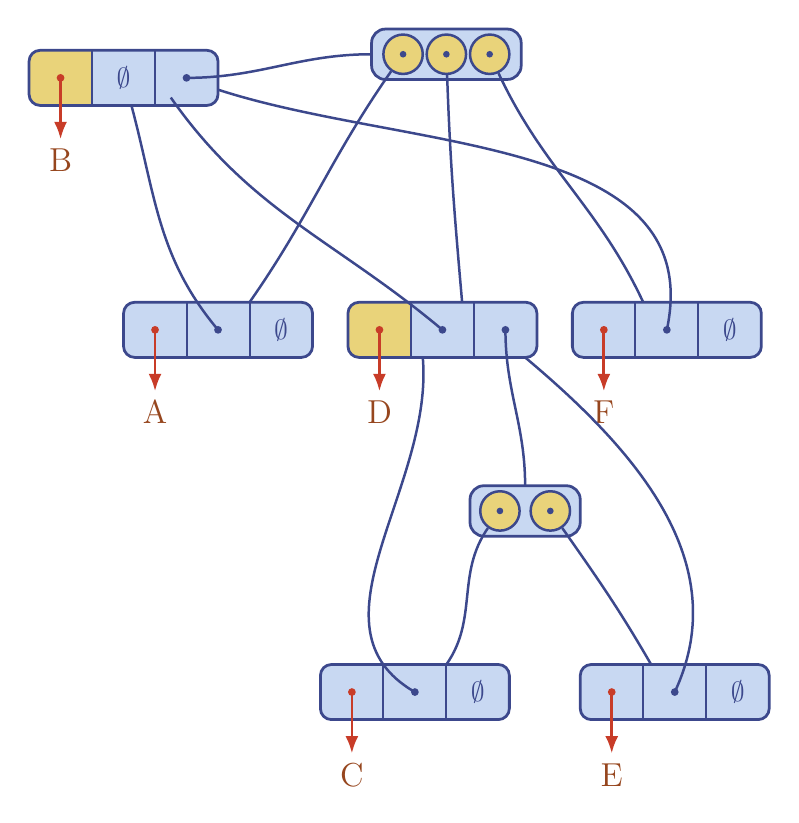
\begin{tikzpicture}[
  ptr/.style={draw=nodeline, line width=0.9pt},
  circ/.style={draw=nodeline, line width=0.9pt, fill=intfill, circle, minimum size=5mm, inner sep=0pt},
]
% ===== Nodes =====
\gtbox{1.3}{8.2}{B}{0}{1}{intfill}    % root: parent null, has children
\gtbox{2.5}{5.0}{A}{1}{0}{leaffill}   % leaf
\gtbox{5.35}{5.0}{D}{1}{1}{intfill}   % internal
\gtbox{8.2}{5.0}{F}{1}{0}{leaffill}   % leaf
\gtbox{5.0}{0.4}{C}{1}{0}{leaffill}   % leaf
\gtbox{8.3}{0.4}{E}{1}{0}{leaffill}   % leaf

% ===== Children container of B (3 circles) =====
\def\Bx{5.4}\def\By{8.5}
\draw[nodeline, line width=1pt, rounded corners=5pt, fill=leaffill]
  ($(\Bx,\By)+(-0.95,-0.32)$) rectangle ($(\Bx,\By)+(0.95,0.32)$);
\node[circ] (bA) at ($(\Bx,\By)+(-0.55,0)$) {};
\node[circ] (bD) at ($(\Bx,\By)+(0,0)$)     {};
\node[circ] (bF) at ($(\Bx,\By)+(0.55,0)$)  {};
\foreach \c in {bA,bD,bF}{\fill[nodeline] (\c) circle (1.2pt);}

% ===== Children container of D (2 circles) =====
\def\Dx{6.4}\def\Dy{2.7}
\draw[nodeline, line width=1pt, rounded corners=5pt, fill=leaffill]
  ($(\Dx,\Dy)+(-0.7,-0.32)$) rectangle ($(\Dx,\Dy)+(0.7,0.32)$);
\node[circ] (dC) at ($(\Dx,\Dy)+(-0.32,0)$) {};
\node[circ] (dE) at ($(\Dx,\Dy)+(0.32,0)$)  {};
\foreach \c in {dC,dE}{\fill[nodeline] (\c) circle (1.2pt);}

% ===== Pointers =====
% Each line begins at an inner field/circle dot; the child link (container ->
% child) and the parent link (child -> parent box) bow apart so they stay clear.
% --- B children-ptr dot -> B container (left border) ---
\draw[ptr] (2.1,8.2) to[out=0,in=180] ($(\Bx,\By)+(-0.95,0)$);
% --- B container circle dots -> child box top (child links) ---
\draw[ptr] (bA) to[out=-125,in=55]  (2.9,5.35);
\draw[ptr] (bD) to[out=-88,in=95]   (5.6,5.35);
\draw[ptr] (bF) to[out=-65,in=115]  (7.9,5.35);
% --- child parent-ptr dot -> B box (parent links, bowed the other way) ---
\draw[ptr] (2.5,5.0) to[out=130,in=-75] (1.4,7.85);   % A.parent -> B
\draw[ptr] (5.35,5.0) to[out=140,in=-55] (1.9,7.95);  % D.parent -> B
\draw[ptr] (8.2,5.0) to[out=78,in=-18]  (2.5,8.05);   % F.parent -> B
% --- D children-ptr dot -> D container (top border) ---
\draw[ptr] (6.15,5.0) to[out=-90,in=90] ($(\Dx,\Dy)+(0.0,0.32)$);
% --- D container circle dots -> child box top (child links) ---
\draw[ptr] (dC) to[out=-125,in=55]  (5.4,0.75);
\draw[ptr] (dE) to[out=-55,in=120]  (8.0,0.75);
% --- child parent-ptr dot -> D box (parent links, bowed the other way) ---
\draw[ptr] (5.0,0.4) to[out=150,in=-85] (5.1,4.65);   % C.parent -> D
\draw[ptr] (8.3,0.4) to[out=65,in=-40]  (6.4,4.65);   % E.parent -> D
\end{tikzpicture}
\end{document}
